%!TEX program = xelatex
\documentclass[10pt]{article}
\usepackage{amssymb}
\usepackage{amsmath}
\usepackage{mathrsfs}
\usepackage{titlesec}
\usepackage{xcolor}
%\usepackage[shortlabels]{enumitem}
\usepackage{enumerate}
\usepackage{bm}
\usepackage{tikz}
\usepackage{listings}
\usetikzlibrary{arrows}
\usepackage{subfigure}
\usepackage{graphicx,booktabs,multirow}
\usepackage[a4paper]{geometry}
\usepackage{upquote}
\usepackage{float}
\usepackage{pdfpages}
\usepackage{amsthm}
\usepackage{bbm}


\geometry{verbose,tmargin=2cm,bmargin=2cm,lmargin=2cm,rmargin=2cm}
\geometry{verbose,tmargin=2cm,bmargin=2cm,lmargin=2cm,rmargin=2cm}
\lstset{language=Matlab}
\lstset{breaklines}

\input defs.tex

\newtheorem{proposition}{Proposition}
\newtheorem{remark}{Remark}

\titleformat*{\section}{\centering\LARGE\scshape}
\renewcommand{\thesection}{\Roman{section}}
\lstset{language=Matlab,tabsize=4,frame=shadowbox,basicstyle=\footnotesize,
keywordstyle=\color{blue!90}\bfseries,breaklines=true,commentstyle=\color[RGB]{50,50,50},stringstyle=\ttfamily,numbers=left,numberstyle=\tiny,
  numberstyle={\color[RGB]{192,92,92}\tiny},backgroundcolor=\color[RGB]{245,245,244},inputpath=code}

\begin{document}

\date{}
\title{CS182, Spring 2022 \\
	Homework 3\\
	\small (Due Tuesday, May. 24 at 11:59pm (CST))}
\maketitle
\begin{enumerate}


	\item \defpoints{15} Given a Bayesian network (Fig.~\ref{fig3}) with five discrete variables $\{F,A,S,H,N\}$,
	      where $\{F,A,S,H,N\}$ are boolean variables.
	      Suppose that $\{F,A,H,N\}$ are observed variables and $\{S\}$ is a latent variable.
	      Now we implement EM algorithm for this model.
	      \begin{figure}[h!]
		      \centering
		      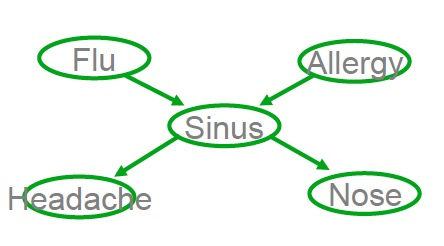
\includegraphics[width=.4\linewidth]{bn.jpg}
		      \label{fig3}
		      \caption{The Bayesian network with five discrete variables $\{F,A,S,H,N\}$.}
	      \end{figure}
	      \begin{itemize}
		      \item[(a)] Derive the E-step. ~\defpoints{5} \\
		      \item[(b)] Derive the M-step. ~\defpoints{5} \\
		      \item[(c)] Guess the solution of parameter estimation in the M-step, according to the MLE solution with all variables being observed. ~\defpoints{5} \\
	      \end{itemize}

\textbf{Solution:}
	\item[\textbf{(a)}]
	      In E-step, we need to compute $P(S|F,A,H,N,\theta)$
	      \\Since $\{F,A,S,H,N\}$ are boolean variables,
	      $$
		      \begin{aligned}
			      P(S_k=0|f_k,a_k,h_k,n_k,\theta) & = \frac{P(S_k=0,f_k,a_k,h_k,n_k|\theta)}{P(S_k=0,f_k,a_k,h_k,n_k|\theta)+P(S_k=1,f_k,a_k,h_k,n_k|\theta)}
		      \end{aligned}
	      $$
	      $$
		      \begin{aligned}
				P(S_k=1|f_k,a_k,h_k,n_k,\theta) & = \frac{P(S_k=1,f_k,a_k,h_k,n_k|\theta)}{P(S_k=0,f_k,a_k,h_k,n_k|\theta)+P(S_k=1,f_k,a_k,h_k,n_k|\theta)}
			  \end{aligned}
	      $$
		  $$
		      \begin{aligned}
				P(S_k=1|f_k,a_k,h_k,n_k,\theta) & =E[s_k]
				  \\&=\frac{P(S_k=1,f_k,a_k,h_k,n_k|\theta)}{P(S_k=0,f_k,a_k,h_k,n_k|\theta)+P(S_k=1,f_k,a_k,h_k,n_k|\theta)}
		      \end{aligned}
	      $$
	\item[\textbf{(b)}]
		In M-step, we need to compute the $\theta'$ which maximize 
		  $$
		      \begin{aligned}
				&E_{P(S|F,A,H,N,\theta)}\log [P(F,A,S,H,N|\theta')]
				\\=&\sum_{k=1}^K \sum_{i=0}^1 P(S_k=i|f_k,a_k,h_k,n_k,\theta) [\log P(f_k)+\log P(a_k)+\log P(s_k|f_k,a_k)+\log P(h_k|s_k)+\log P(n_k|s_k)]
		      \end{aligned}
	      $$
	\item[\textbf{(c)}]MLE solution:
			$$\theta_{f} =\frac{\sum_{k=1}^{K} \delta\left(f_{k}=1\right)}{K}$$
			$$\theta_{a} =\frac{\sum_{k=1}^{K} \delta\left(a_{k}=1\right)}{K}$$
			$$\theta_{s \mid f, a} =\frac{\sum_{k=1}^{K} \delta\left(s_{k}=s,f_{k}=f, a_{k}=a\right)}{\sum_{k=1}^{K} \delta\left(f_{k}=f, a_{k}=a\right)}$$
			$$\theta_{h \mid s} =\frac{\sum_{k=1}^{K} \delta\left(h_{k}=1,s_{k}=s\right) }{\sum_{k=1}^{K} \delta\left(s_{k}=s\right)}$$
			$$\theta_{n \mid s} =\frac{\sum_{k=1}^{K} \delta\left(n_{k}=1,s_{k}=s\right) }{\sum_{k=1}^{K} \delta\left(s_{k}=s\right)}$$
	      M-step solution:
		    $$\theta_{f} =\frac{\sum_{k=1}^{K} \delta\left(f_{k}=1\right)}{K}$$
			$$\theta_{a} =\frac{\sum_{k=1}^{K} \delta\left(a_{k}=1\right)}{K}$$
			$$\theta_{s \mid f, a} =\frac{\sum_{k=1}^{K}  \delta\left(f_{k}=f, a_{k}=a\right)P\left(s_{k}=s\right)}{\sum_{k=1}^{K} \delta\left(f_{k}=f, a_{k}=a\right)}$$
			$$\theta_{h \mid s} =\frac{\sum_{k=1}^{K} \delta\left(h_{k}=1\right) P\left(s_{k}=s\right)}{\sum_{k=1}^{K} P\left(s_{k}=s\right)}$$
			$$\theta_{n \mid s} =\frac{\sum_{k=1}^{K} \delta\left(n_{k}=1\right) P\left(s_{k}=s\right)}{\sum_{k=1}^{K} P\left(s_{k}=s\right)}$$
			\newpage

	\item \defpoints{20}
	      Suppose two data points($x_1 = 0$, $x_2 = 1$) are generated from two Gaussian mixture model(A and B).The parameter of the two Gaussian model are unknown. We want to use EM to guess parameters of the two Gaussian models. For simplicity, the priors are set to equal, which means $P(a) = P(b) = \frac{1}{2}$.
	      EM can be divided into following steps:
	      \begin{enumerate}
		      \item Randomly choose $(\mu_a, \sigma_a^2)$ and $(\mu_b, \sigma_b^2)$.
		      \item For each point $x_i$, calculate $P(a|x_i)$ and $P(b|x_i)$.
		      \item Adjust $(\mu_a, \sigma_a^2)$ and $(\mu_b, \sigma_b^2)$.
		      \item Repeat 2 and 3 until convergence.
	      \end{enumerate}
	      Suppose we randomly choose parameters as: $(\mu_a, \sigma_a^2) = (0, 1)$ and $(\mu_b, \sigma_b^2) = (1, 1)$

	      \begin{enumerate}
		      \item[(1)] E-step: calculate $P(a|x_i)$ and $P(b|x_i)$, $i = 1, 2$.\defpoints{10}\\
		      \item[(2)] M-step: Adjust $(\mu_a, \sigma_a^2)$ and $(\mu_b, \sigma_b^2)$ with following formula.\defpoints{10} \\
		            $$\mu_a = \frac{a_1x_1 + a_2x_2}{a_1 + a_2}, \qquad \sigma_a^2 = \frac{a_1(x_1-\mu_a)^2 + a_2(x_2-\mu_a)^2}{a_1 + a_2}$$
		            where $a_1 = P(a|x_1)$ and $a_2 = P(a|x_2)$\\
	      \end{enumerate}
\textbf{Solution:}
	\item[\textbf{(1)}]
		$$
		\begin{aligned}
		P(a|x_i)&=P\left(a \mid x_{i}\right)
		\\&=\frac{P\left(x_{i} \mid a\right)  P(a)}{P\left(x_{i}\right)}
		\\&=\frac{1}{2}\frac{P\left(x_{i} \mid a\right)}{P\left(x_{i} \mid a\right)  P(a)+P\left(x_{i} \mid b\right)  P(b)}
		\\&=\frac{P\left(x_{i} \mid a\right)}{P\left(x_{i} \mid a\right)+P\left(x_{i} \mid b\right)}
		\end{aligned}
		$$
	    similarly,$$P(b|x_i)=\frac{P\left(x_{i} \mid b\right)}{P\left(x_{i} \mid a\right)+P\left(x_{i} \mid b\right)}$$
		By Gaussian mixture model, we know
		$$P\left(x_{i} \mid a\right)=\frac{1}{\sigma_a \sqrt{2 \pi}} e^{-\frac{(x_i-\mu_a)^{2}}{2 \sigma_a^{2}}}$$
		$$P\left(x_{i} \mid b\right)=\frac{1}{\sigma_b \sqrt{2 \pi}} e^{-\frac{(x_i-\mu_b)^{2}}{2 \sigma_b^{2}}}$$
		Bringing in the values gives,
		$$P\left(a \mid x_{1}\right)=\frac{1}{1+e^{-\frac{1}{2}}}$$
		$$P\left(b \mid x_{1}\right)=\frac{e^{-\frac{1}{2}}}{1+e^{-\frac{1}{2}}}$$
		$$P\left(a \mid x_{2}\right)=\frac{e^{-\frac{1}{2}}}{1+e^{-\frac{1}{2}}}$$
		$$P\left(b \mid x_{2}\right)=\frac{1}{1+e^{-\frac{1}{2}}}$$

	\item[\textbf{(2)}]
 		$a_1=P(a|x_1)=\frac{1}{1+e^{-\frac{1}{2}}}$,
		$a_2=P\left(a \mid x_{2}\right)=\frac{e^{-\frac{1}{2}}}{1+e^{-\frac{1}{2}}}$
		$$
		\begin{aligned}
		\mu_a&=\frac{a_1x_1 + a_2x_2}{a_1 + a_2}
		\\&=\frac{a_2}{a_1 + a_2}
		\\&=a_2
		\\&=\frac{e^{-\frac{1}{2}}}{1+e^{-\frac{1}{2}}}
		\end{aligned}
		$$
		$$
		\begin{aligned}
		\sigma_a^2 &= \frac{a_1(x_1-\mu_a)^2 + a_2(x_2-\mu_a)^2}{a_1 + a_2}
		\\&=a_1\mu_a^2 + a_2(1-\mu_a)^2
		\\&=\frac{e^{-\frac{1}{2}}}{(1+e^{-\frac{1}{2}})^2}
		\end{aligned}
		$$
		$b_1=P\left(b \mid x_{1}\right)=\frac{e^{-\frac{1}{2}}}{1+e^{-\frac{1}{2}}}$,
		$b_2=P\left(b \mid x_{2}\right)=\frac{1}{1+e^{-\frac{1}{2}}}$
		$$
		\begin{aligned}
		\mu_b&=\frac{b_1x_1 + b_2x_2}{b_1 + b_2}
		\\&=\frac{b_2}{b_1 + b_2}
		\\&=b_2
		\\&=\frac{1}{1+e^{-\frac{1}{2}}}
		\end{aligned}
		$$
		$$
		\begin{aligned}
		\sigma_b^2 &= \frac{b_1(x_1-\mu_b)^2 + b_2(x_2-\mu_b)^2}{b_1 + b_2}
		\\&=b_1\mu_b^2 + b_2(1-\mu_b)^2
		\\&=\frac{e^{-\frac{1}{2}}}{(1+e^{-\frac{1}{2}})^2}
		\end{aligned}
		$$
		 \newpage

	\item ~\defpoints{30}
	      Suppose that we are interested in learning a classifier, such that at any turn of a game we can pose a question, like "should I attack this ant hill now?", and get an answer.That is, we want to build a classifier which we can feed some features on the current game state, and get the output "attack" or "don't attack". There are many possible ways to define what the action "attack" means, but for now let's define it as sending all friendly ants that can see the ant hill under consideration towards it.

	      Let’s recall the AdaBoost algorithm described in class. Its input is a dataset $\{(x_{i},y_{i})\}_{i=1}^{n}$, with $x_i$ being the $i$-th sample, and $y_{i}\in \{-1,1\}$ denoting the $i$-th label, $i=1,2,...,n$. The features might be composed of a count of the number of friendly ants that can see the ant hill under consideration, and a count of the number of enemy ants these friendly ants can see. For example, if there were 10 friendly ants that could see a particular ant hill, and 5 enemy ants that the friendly ants could see, we would have:
	      \begin{align*}
		      x_1 = \begin{bmatrix}
			      10 \\
			      5
		      \end{bmatrix}.
	      \end{align*}

	      The label of the example $x_{1}$ is $y_{1} = 1$, once the friendly ants were successful in razing the enemy ant hill, and $y_{1} = 0$ otherwise. We could generate such examples by running a greedy bot (or any other opponent bot) against a bot that we make periodically try to attack an enemy ant hill. Each time this bot tries the attack, we record (say, after $20$ turns or some other significant amount of time) whether the attack was successful or not.

	      \begin{itemize}
		      \item[(a)] Let $\epsilon_t$ denote the error of a weak classifier $h_t$:
		            \begin{align*}
			            \epsilon_{t} = \sum_{i=1}^{n} D_{t}(i) \mathbbm{1}(y_{i} \neq h_{t}(x_{i})).
		            \end{align*}
		            In the simple “attack” / “don’t attack” scenario, suppose that we have implemented the following six weak classifiers:
		            \begin{align*}
			            h^{(1)}(x_{i}) = 2 * \mathbbm{1}(x_{i1} \geq 2) - 1, \hspace{1cm}  & h^{(4)}(x_{i}) = 2 * \mathbbm{1}(x_{i2} \leq 2) - 1,  \\
			            h^{(2)}(x_{i}) = 2 * \mathbbm{1}(x_{i1} \geq 6) - 1, \hspace{1cm}  & h^{(5)}(x_{i}) = 2 * \mathbbm{1}(x_{i2} \leq 6) - 1,  \\
			            h^{(3)}(x_{i}) = 2 * \mathbbm{1}(x_{i1} \geq 10) - 1, \hspace{1cm} & h^{(6)}(x_{i}) = 2 * \mathbbm{1}(x_{i2} \leq 10) - 1. \\
		            \end{align*}
		            Given ten training data points ($n = 10$) as shown in Table 1,
		            \begin{table}[t]
			            \caption{The training data in (a).}
			            \label{table1}
			            \centering
			            \begin{tabular}{|c|cc|c|}
				            \hline
				            $i$ & $x_{i1}$ & $x_{i2}$ & $y_{i}$ \\ \hline
				            1   & 1.5      & 0.5      & 1       \\
				            2   & 2.5      & 1.5      & 1       \\
				            3   & 3.5      & 3.5      & 1       \\
				            4   & 6.5      & 5.5      & 1       \\
				            5   & 7.5      & 10.5     & 1       \\
				            6   & 1.5      & 2.5      & -1      \\
				            7   & 3.5      & 1.5      & -1      \\
				            8   & 5.5      & 5.5      & -1      \\
				            9   & 7.5      & 8.5      & -1      \\
				            10  & 1.5      & 10.5     & -1      \\
				            \hline
			            \end{tabular}
		            \end{table}
		            please show that what is the minimum value of $\epsilon_{1}$ and which of $h^{(1)},...,h^{(6)}$ achieve this value? Note that there may be multiple classifiers that all have the same $\epsilon_{1}$. You should list all classifiers that achieve the minimum $\epsilon_{1}$ value.~\defpoints{6}\\

		      \item[(b)] For all the questions in the remainder of this section, let $h_{1}$ denote $h^{(1)}$ chosen in the first round of boosting. (That is, $h^{(1)}$ was the classifier that achieved the minimum $\epsilon_{1}$.)
		            \begin{enumerate}
			            \item[(1)] What is the value of $\alpha_{1}$ (the weight of this first classifier $h_{1}$)? ~\defpoints{2}\\

			            \item[(2)] What should $Z_{t}$ be in order to make sure the distribution $D_{t+1}$ is normalized correctly? That is, derive the formula of $Z_{t}$ in terms of $\epsilon_{t}$ that will ensure $\sum_{i=1}^{n} D_{t+1}(i) = 1$. Please aslo derive the formula of $\alpha_{t}$ in terms of $\epsilon_{t}$. ~\defpoints{6}\\

			            \item[(3)] Which points will increase in significance in the second round of boosting? That is, for which points will we have $D_{1}(i) < D_{2}(i)$? What are the values of $D_{2}$ for these points?~\defpoints{5}\\

			            \item[(4)] In the second round of boosting, the weights on the points will be different, and thus the error $\epsilon_2$ will also be different. Which of $h^{(1)}, . . . , h^{(6)}$ will minimize $\epsilon_2$? (Which classifier will be selected as the second weak classifier $h_2$?) What is its value of $\epsilon_2$?~\defpoints{6}\\

			            \item[(5)] What will the average error of the final classifier $H$ be, if we stop after these two rounds of boosting? That is, if $H(x) = \text{sign}(\alpha_{1}h_{1}(x) + \alpha_{2}h_{2}(x))$, what will the  training error $\epsilon = \frac{1}{n} \sum_{i=1}^{n} \mathbbm{1} (y_{i} \neq h(x_{i}))$ be? Is this more, less, or the same as the error we would get, if we just used one of the weak classifiers instead of this final classifier $H$?~\defpoints{5}\\

		            \end{enumerate}
	      \end{itemize}
\textbf{Solution:} 	
		\item[\textbf{(a)}]		
		By six different weak classifiers, the $\epsilon_1$ values of $h^{(1)},...,h^{(6)}$ is $4/10,4/10,5/10,4/10,4/10,5/10$ which equals $0.4,0.4,0.5,0.4,0.4,0.5$
		\\the minimum one is $0.4$, the 1st, 2nd, 4th, 5th classifiers achieve the minimum.
		\item[\textbf{(b)}]	
			\item[\textbf{(1)}]
		  	Using formula $$\alpha_{t}=\frac{1}{2} \ln \left(\frac{1-\epsilon_{t}}{\epsilon_{t}}\right)$$
			Then, 
			  $$
			  \begin{aligned}
				\alpha_{1}&=\frac{1}{2} \ln \left(\frac{1-\epsilon_{1}}{\epsilon_{1}}\right)
				\\&=\frac{1}{2}\ln \left(\frac{3}{2}\right)
				\\&\approx 0.2027
			  \end{aligned}
			  $$
			\item[\textbf{(2)}]
			  Since $D_{t+1}(i)=\frac{D_{t}(i)}{Z_{t}} \mathrm{e}^{\left\{-\alpha_{t} y_{i} h_{t}\left(x_{i}\right)\right\}}$
			  $$
			  \begin{aligned}
				D_{t+1}(i)&=\frac{D_{t}(i)}{Z_{t}} \mathrm{e}^{\left\{-\alpha_{t} y_{i} h_{t}\left(x_{i}\right)\right\}}
				\\1=\sum_{i=1}^nD_{t+1}(i)&=\sum_{i=1}^n\frac{D_{t}(i)}{Z_{t}} \mathrm{e}^{\left\{-\alpha_{t} y_{i} h_{t}\left(x_{i}\right)\right\}}
				\\Z_t&=\sum_{i=1}^nD_{t}(i)\mathrm{e}^{\left\{-\alpha_{t} y_{i} h_{t}\left(x_{i}\right)\right\}}
			  \end{aligned}
			  $$
			  Since
			  $$
			  \begin{aligned}
			  &D_{t+1}(i)=\frac{D_{t}(i)}{Z_{t}} \mathrm{e}^{\left\{-\alpha_{t}\right\}} \text { if } y_{i}=h_{t}\left(x_{i}\right) \\
			  &D_{t+1}(i)=\frac{D_{t}(i)}{Z_{t}} \mathrm{e}^{\left\{\alpha_{t}\right\}} \text { if } y_{i} \neq h_{t}\left(x_{i}\right)
			  \end{aligned}
			  $$
			  $$
			  \begin{aligned}
				Z_t&=\sum_{i=1}^nD_{t}(i)\mathrm{e}^{\left\{-\alpha_{t} y_{i} h_{t}\left(x_{i}\right)\right\}}
				\\&=\sum_{y_i=h_t(x_i)}D_{t}(i)\mathrm{e}^{\left\{-\alpha_{t} \right\}}+\sum_{y_i\neq h_t(x_i)}D_{t}(i)\mathrm{e}^{\left\{\alpha_{t} \right\}}
				\\&=(1-\epsilon_t)\mathrm{e}^{\left\{-\alpha_{t} \right\}}+\epsilon_t\mathrm{e}^{\left\{\alpha_{t} \right\}}
			\end{aligned}
			  $$
			  To minimize the training error,
			  $$
			  \begin{aligned}
				\alpha_t&=\underset{\alpha}{\argmin}[(1-\epsilon_t)\mathrm{e}^{\left\{-\alpha_{t} \right\}}+\epsilon_t\mathrm{e}^{\left\{\alpha_{t} \right\}}]
			  \end{aligned}
			  $$
			  By $\frac{\partial Z_t}{\partial \alpha_t}=0$, we know $\alpha_{t}=\frac{1}{2} \ln \left(\frac{1-\epsilon_{t}}{\epsilon_{t}}\right)$.
			  Then, $Z_t=2\sqrt{\epsilon_t(1-\epsilon_t)}$

			\item[\textbf{(3)}]The points which misclassifies will increase in weight in $D_2$. 
			They are 1st, 7th, 8th, 9th ($i=1,7,8,9$) points. For these points,
			  $$
			  \begin{aligned}
				D_{2}(i) &=\frac{D_{1}(i) \exp \left(-\alpha_{t} y_{i} h_{t}\left(x_{i}\right)\right)}{Z_{t}} \\
				&=\frac{\frac{1}{10}\exp \{\alpha_{1}\}}{4 * \exp \{\alpha_{1}\}+6 * \exp \{-\alpha_{1}\}} \\
				&=\frac{1}{8}
			  \end{aligned}
			  $$
			  which means $D_2(1)=D_2(7)=D_2(8)=D_2(9)=\frac{1}{8}$
			\item[\textbf{(4)}]
			  By (3), similarly, for $i=2,3,4,5,6,10$, $D_2(i) = \frac{1}{12}$.
			  \\the error values of $\epsilon_2$ for $h^{(1)},...,h^{(6)}$ is 
			  $\frac{4}{8},\frac{2}{8}+\frac{2}{12},\frac{1}{8}+\frac{4}{12},\frac{1}{8}+\frac{3}{12},\frac{2}{8}+\frac{2}{12},\frac{3}{8}+\frac{2}{12}$
			  which equals $\frac{1}{2},\frac{5}{12},\frac{11}{24},\frac{3}{8},\frac{5}{12},\frac{13}{24}$
			  \\Thus,$h_4$ will minimize $\epsilon_2$, the value is $\frac{3}{8}$.
			  \item[\textbf{(5)}]
			  By (4) and (2), $\alpha_2 = \frac{1}{2} \ln \left(\frac{1-\epsilon_{2}}{\epsilon_{2}}\right)=\frac{1}{2}\ln \frac{7}{5}$
			  \\Thus,
			  $$
			  \begin{aligned}
				H(x)&= \text{sign}(\alpha_{1}h_{1}(x) + \alpha_{2}h_{4}(x))
				\\&=\text{sign}(h_{1}(x)\ln \frac{3}{2} + h_{4}(x)\ln \frac{7}{5})
			  \end{aligned}
			  $$
			  Since $\alpha_1!=\alpha_2$ and $h_t(x_i)=1$ or $-1$, $H(x)$ equals to one of $h_1(x),h_4(x)$
			  ($H(x)= \text{sign}(\alpha_{1}h_{1}(x) + \alpha_{2}h_{4}(x))$ sign of it is only about the large coefficient one $h_t(x)$)
			  \\Since $\alpha_1>\alpha_2$, we know $H(x)=h_1(x)$, which means $\epsilon = \epsilon_1 = 0.4$

			\newpage

	\item ~\defpoints{15}
	      Given valid kernels $k_1(\mathbf{x}, \mathbf{x}')$ and $k_2(\mathbf{x}, \mathbf{x}')$, please verify the following new kernels will also be valid:
	      \begin{enumerate}
		      \item $k\left(\mathbf{x}, \mathbf{x}^{\prime}\right)=f(\mathbf{x}) k_{1}\left(\mathbf{x}, \mathbf{x}^{\prime}\right) f\left(\mathbf{x}^{\prime}\right)$, where $f(\cdot)$ is any function. ~\defpoints{5}
		      \item $k(\mathbf{x}, \mathbf{x}^\prime) = q(k_1(\mathbf{x}, \mathbf{x}^\prime))$, where $q(\cdot)$ is a polynomial with nonnegative coefficients. ~\defpoints{5}
		      \item $k(\mathbf{x}, \mathbf{x}^\prime) = \mathbf{x^\top}\mathbf{Ax}^\prime$, where $\mathbf{A}$ is a symmetric positive semi-definite matrix.~\defpoints{5}
	      \end{enumerate}
\textbf{Solution:}
		  \item[\textbf{(a)}]
			Since $k_1(x,x')$ can be written as $<\phi(x),\phi(x')>$,
				$$
				\begin{aligned}
					k(x,x')=f(x)\phi(x)^T\phi(x')f(x')=<\phi(x)f(x)^T,\phi(x')f(x')>
				\end{aligned}
				$$
			it can be written as inner product of feature vectors, so it is valid kernel.
		  \item[\textbf{(b)}]
			  First,product of valid kernels is valid kernel, sum of valid kernels is valid kernel.
			  \\So,$$q(x)=\sum_{i=1}^n a_n x^n$$
			  $$
				\begin{aligned}
					k(x,x')=\sum_{i=1}^n a_n (k_1(x,x')^n)
				\end{aligned}
			  $$
			  Thus, it is a valid kernel.
		  \item[\textbf{(c)}]
			Eigendecomposition of $A$ is $Q\Lambda Q^T$, and  $\Lambda$ is diagonal matrix.
			So,
			$$
				\begin{aligned}
					k(x,x')&=x^T A x'
					\\&= x^T Q\Lambda Q^T x
					\\&=(\Lambda^{0.5}Q^Tx)^T(\Lambda^{0.5}Q^Tx')
					\\&=<(\Lambda^{0.5}Q^Tx),(\Lambda^{0.5}Q^Tx')>
				\end{aligned}
			$$ 
			it can be written as inner product of feature vectors, so it is valid kernel.
	      \newpage

	\item ~\defpoints{20} We have learned that when solving a SVM problem, we need to first construct Lagrangian function $L(w,b,\alpha)$ and set partial derivative to zero. By using KKT conditions, we can get the dual problem of SVM :
	      \begin{align*}
		       & \underset{\alpha}{min} \  \frac{1}{2}\sum\limits_{i=1}^{n}\sum\limits_{j=1}^{n}\alpha_i \alpha_j y_i y_j <x_i,x_j> - \sum\limits_{i=1}^{n}\alpha_i , \\ & \ \ \ \ \ \ \  s.t. \ \alpha_i \geq 0 , \ \ \ \ \sum\limits_{i=1}^{n}\alpha_i y_i = 0
	      \end{align*}
	      Now we use a simple example to better understand how SVM works. We consider the separating hyperplane being $wx + b = 0$. Suppose we have three data points: $x_1 = (2,-1)^T, x_2 = (2,-3)^T, x_3 = (4,-1)^T$, the corresponding labels are: $y_1 = -1, y_2 = -1, y_3 = 1$. Use SVM to find the the values of $w^* = (w_1^*, w_2^*)$, $b^*$ and give the separating hyperplane. Please show your calculation process.

\textbf{Solution:}
	\\First, $y_1 = -1, y_2 = -1, y_3 = 1$, so $\alpha_1+\alpha_2-\alpha_3=0$.
	\\Then by $\underset{\alpha}{min} \  \frac{1}{2}\sum\limits_{i=1}^{n}\sum\limits_{j=1}^{n}\alpha_i \alpha_j y_i y_j <x_i,x_j> - \sum\limits_{i=1}^{n}\alpha_i$,
		\\we know
			$$
				\begin{aligned}
					\alpha&=\underset{\alpha}{min} \  \frac{1}{2}\sum\limits_{i=1}^{n}\sum\limits_{j=1}^{n}\alpha_i \alpha_j y_i y_j <x_i,x_j> - \sum\limits_{i=1}^{n}\alpha_i
					\\&=\underset{\alpha}{min} \  5\alpha_2^2+2\alpha_3^2-2\alpha_3
				\end{aligned}
			$$ 
	Thus, $\alpha_2=0$ and $\alpha_3=\frac{1}{2}$,$\alpha_1=\frac{1}{2}$.
	$$
		\begin{aligned}
			w*&=\sum_i \alpha_i y_i x_i
			\\&=(1,0)
		\end{aligned}
	$$
	$y_i=w*x_i+b\Rightarrow b*=-3$
	\\the separating hyperplane: $0=x_1-3$
\end{enumerate}





\end{document}
